\section{HTTP/2}

HTTP/2 surge para solucionar problemas de HTTP/1.1. Entre ellos, tenemos los siguientes.

\begin{itemize}[label=\textcolor{acento}{$\bullet$}]
    \item Protocolo sincrónico
    \item Tiene head-of-line blocking
    \item Requiere múltiples conexiones a un servidor para utilizar paralelismo
\end{itemize}

\begin{definicion}{Descripción General}
    Protocolo de capa de aplicación orientado a conexión, se ejecuta sobre TCP y sus conexiones son persistentes. El cliente no debería abrir más de una conexión TCP al servidor.
    
    Se introducen nuevos conceptos:
    \begin{enumerate}
        \item \textbf{Stream:} flujo bidireccional de frames dentro de \textbf{una conexión}.
        \item \textbf{Frame:} unidad básica del protocolo, cada tipo de frame sirve un propósito diferente y un frame pertenece a un stream en particular.
    \end{enumerate}

    A diferencia de HTTP/1.1 que era de texto plano HTTP/2 es \textbf{binario}, lo que lo hace incompatible con otras versiones de HTTP. 

    Utiliza los mismos puertos que HTTP/1.1 (puerto 80 y 443 para HTTPS).
\end{definicion}

Para utilizar HTTP/2, es necesario verificar si el otro extremo también soporta este protocolo.

\subsection{Frames}

Son la unidad más pequeña que trasnporta todos los datos (headers, payload, etc.). Además de tener los campos de una cabecera tradicional (length, type, flags) también agrega el \textbf{Stream Identifier} para indicar a qué stream pertenece el frame. 

Hay distintos tipos de frames.

\begin{itemize}[label=\textcolor{acento}{$\bullet$}]
    \item \textbf{HEADERS:} usado para abrir un stream, transporta cabeceras del requerimiento y/o respuesta.
    \item \textbf{DATA:} transporta bytes de longitud variable asociados a un stream.
    \item \textbf{RST\_STREAM:} cierra el stream inmediatamente. El emisor no envía nuevos frames, pero si puede recibir.
    \item \textbf{SETTINGS:} transporta parámetros de configuración que afectan a la conexión. Se envían solo en el primer stream, y debe ser enviado por cada extremo.
    \item \textbf{PUSH\_PROMISE:} solo los envía el servidor, sirven para avisar de streams que el emisor va a utilizar.
    \item \textbf{PING:} mide el RTT y determina si la cinexión aún está activa.
    \item \textbf{GOAWAY:} inicia el cierre elegante de una conexión o indica conexiones de error.
    \item \textbf{WINDOWS\_UPDATE:} se utiliza para controlar el flujo en los streams o conexión.
\end{itemize}

\subsection{Streams}

\begin{definicion}{Definición}
    Secuencia bidireccional de frames intercambiados entre cliente y servidor de una conexión. Pueden haber varios abiertos concurrentemente, cada uno identificado con un entero asignado por el extremo que lo inicia. Si lo hace el servidor, es par. Sino es impar. Importa el orden en el que se envían los frames, ya que se procesan en ese orden.
\end{definicion}

El stream con \textbf{identificador 0} se utilza para enviar mensajes de \textbf{control de conexión}. Cada nuevo identificador debe ser mayor a todos los elegidos previamente por ese extremo.

Si un cliente envía una solicitud HTTP en un nuevo stream, el servidor envía la respuesta en ese mismo stream de la solicitud. Cada una de ellas puede consistir de uno o más frames.

Una \textbf{solicitud o respuesta HTTP/2} consta de un frame \texttt{HEADER} y cero o más frames \texttt{DATA}.

\begin{figure}[H]
    \centering
    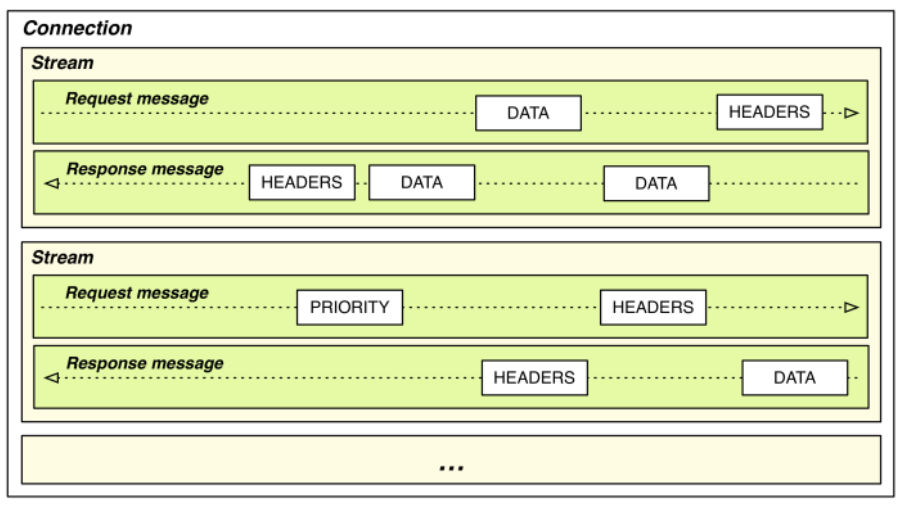
\includegraphics[width=0.8\textwidth]{capitulos/http2/imagenes/conexion.png}
    \caption{Conexiones en HTTP/2}
    \label{fig:http2-conexion}
\end{figure}

\begin{figure}[H]
    \centering
    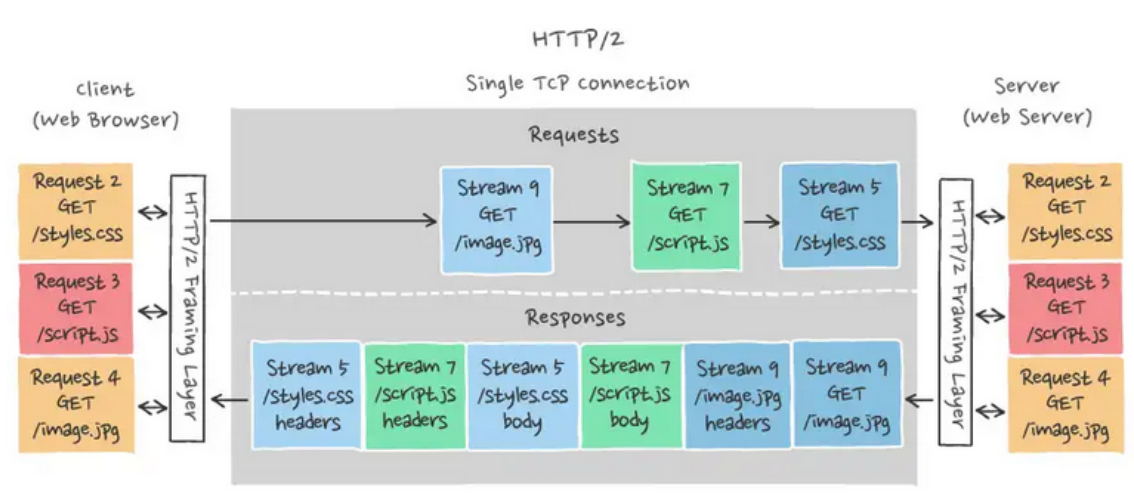
\includegraphics[width=0.8\textwidth]{capitulos/http2/imagenes/conexion-2.png}
    \caption{Conexiones en HTTP/2 - 2}
    \label{fig:http2-conexion-2}
\end{figure}

\subsection{Control de Flujo}

Los streams \textbf{compiten entre sí} por el uso de la conexión TCP. Como TCP no puede aplicar control de flujo sobre los streams individuales, cada emisor debe mantener una \textbf{ventana por cada stream}.

\begin{definicion}{Capacidad de Buffering}  
    Valor entero que indica cuantos bytes de datos puede transmitir el emisor. Es unidireccional: cada extremo anuncia su tamaño máximo de ventana para la conexión y cada stream.
\end{definicion}

El \textbf{frame \texttt{SETTINGS}} permite modificar el tamaño de la ventana al \textbf{inicio} de la conexión (el tamaño default es 65.535 bytes), y el límite sólo se aplica sobre los frames \texttt{DATA}.

\begin{nota}{\emph{Recordar...}\smallskip}
    El \texttt{WINDOW\_UPDATE} puede ser específico para un stream o para la conexión entera, ya que se mantiene una \textbf{ventana por cada stream} y para la \textbf{conexión como un todo}.
\end{nota}

\subsection{Server Push}

Consiste en que el servidor puede enviar un recurso antes de que el cliente se lo solicite, mandando un \textbf{frame \texttt{PUSH\_PROMISE}}. Dentro de este push promise se indica cual es el identificador de stream que se usará para la respuesta.

\begin{figure}[H]
    \centering
    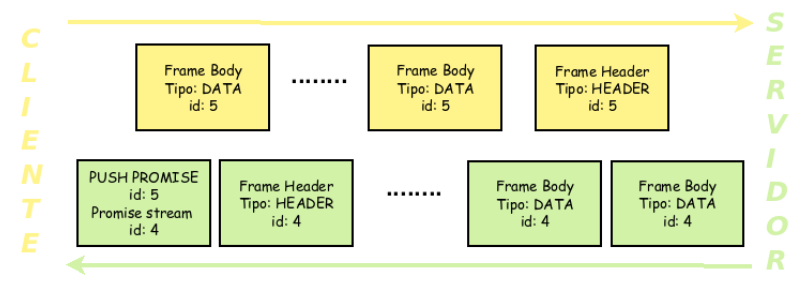
\includegraphics[width=0.8\textwidth]{capitulos/http2/imagenes/server-push.png}
    \caption{Server push}
    \label{fig:http2-server-push}
\end{figure}

\subsection{Head Compression}

En HTTP/1.1 podíamos comprimir solo el payload. En HTTP/2 podemos \textbf{comprimir la cabecera y el payload} utilizando \emph{\textbf{HPACK}}, que es un algoritmo de compresión diseñado para comprimir cabeceras. Consiste en una tabla estática predefinida y una tabla dinámica que permite agregar cabeceras a continuación de la estática.

\begin{figure}[H]
    \centering
    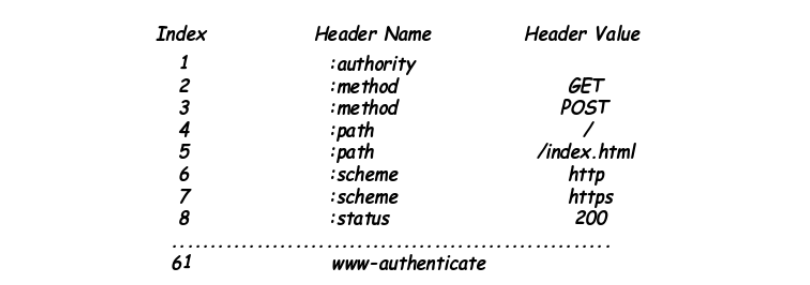
\includegraphics[width=0.8\textwidth]{capitulos/http2/imagenes/hpack.png}
    \caption{HPACK}
    \label{fig:http2-hpack}
\end{figure}